\Subhead{2.9.1}{Уравнения Кортевега--де-Вриза и синус--Гордона. Стационарные волны. Понятие о солитонах}

Дисперсия может уравновесить нелинейное укручение без необратимых потерь. Нормированное уравнение Кортевега–де–Вриза
\begin{equation}
 u_t+6uu_x+u_{xxx}=0
\end{equation}
имеет локализованное решение $u(x,t)=U(\xi)$, $\xi=x-Vt$. После одного интегрирования с нулевыми значениями на бесконечности $U''=VU-3U^2$; умножение на $U'$ даёт $(U')^2=VU^2-2U^3$. Поэтому
\begin{equation}
 u=\frac V2\operatorname{sech}^2\left[\frac{\sqrt V}{2}(x-Vt-x_0)\right],\quad V>0.
\end{equation}
Большая амплитуда соответствует большей скорости и меньшей ширине. Это баланс дисперсии и нелинейности, а не диссипативный ударный фронт.

Нормированное уравнение синус–Гордона $\phi_{tt}-\phi_{xx}+\sin\phi=0$ описывает, например, фазу в длинном джозефсоновском переходе. Его кинк
\begin{equation}
 \phi=4\arctan\exp\left[\frac{x-vt-x_0}{\sqrt{1-v^2}}\right],\qquad |v|<1,
\end{equation}
соединяет эквивалентные минимумы $0$ и $2\pi$ и имеет топологический заряд. Единица скорости здесь — характеристическая скорость выбранной нормировки.

Уединённая волна сохраняет форму при движении; термин «солитон» дополнительно подчёркивает особые свойства взаимодействия в интегрируемой модели: после столкновения восстанавливаются формы и скорости, остаются фазовые/координатные сдвиги. Не всякая локализованная волна реальной среды обладает этой точной упругостью.
\begin{center}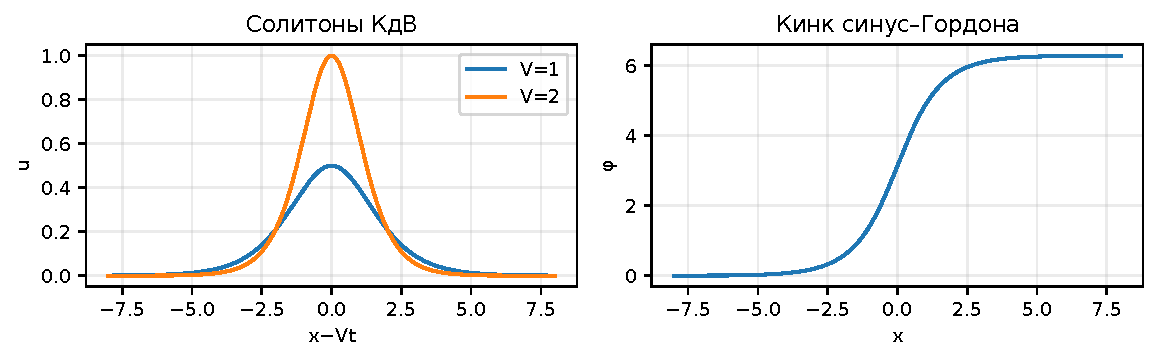
\includegraphics[width=0.8\linewidth]{figures/soliton.pdf}\end{center}

